\chapter{Application}
\label{ch:Allpication}

The listed algorithms have their theoretical benefits, but they might not be good for real issues. The numeric obstacles require the trade-offs between robustness, stability, and calculation time. The computer memory has limited capacity; systems discretization adds the plant errors. We considered the examples do not have a physical reference system. Now, we try to apply the algorithms on the more ''real'' plant and see the problems that occur. 


\section{The case $D = 0$}
		\begin{exam}
		 We consider a dynamical system, which describes a flexible satellite. As known from \cite{SchRC} the continuous-time transfer function has the form  
		\begin{align}
		G(s) = \frac{.036(s + 25.28)}{s^2(s^2 + .0396s + 1)}. 
		\end{align}
	
		
		Since we are working with discrete time systems, we discretize it for sample time $T_s = 10^{-3}$  and get the state space description 
		\begin{align}
		\label{eq:Appl:satellite_sys}
		\left( \begin{array}{c | c}
		A & B \\ \hline C & D
		\end{array}\right) = 
		\left(\begin{array}{c c c c | c}
	    1.000  &  0.005  &  0.000  &  0.000 & 1.047\cdot 10^{-13}\\
		0  &  1.000  &  0.001  &  0.000 & 8.333\cdot 10^{-11}\\
		0  &       0  &  1.000  &  0.001 & 2.5\cdot 10^{-7}\\
		0  &       0  & -0.001  &  1.000 & 5\cdot 10^{-4}\\ \hline
        0.362 & 0.072&  0 & 0 & 0
		\end{array}\right). 
	\end{align}
	\end{exam}

In this example, the matrix $D$ is zero, what makes our algorithms not applicable. 
Moreover, the  $D$-part's neglecting is typical: the system output must mostly image the system state and not the known input we send. 

Let us consider the output signal at time $1\leq t \leq N$:
\begin{align}
y(t) = C x(t) = CA x(t) + C B u(t).
\end{align}

Here the ''new'' $D$-term is represented by the matrix $CB$, if it is not zero. 
With other words, the input $u(t)$ begins to impact the output after the first time step. We say, that the  \textit{relative degree} of the system equals 1. We define it mathematically precise: 
\begin{defi}
	The relative degree of the system $(A, B, C, D)$ is 0 if $D \neq 0$. For $D = 0$ it is the smallest integer $k^*$ for which $	C A^{k^*-1} B \neq 0$.
\end{defi} 

We put the first $k^*$ terms away and consider our dynamical system from time step $k^*$
\begin{align}
\begin{split}
x(t+1) &= A x(t) + B u(t), \\
y(t) &= C A^{k^* + 1}x(t) + C A^{k^*} B u(t),  \text{ for } t = k^*, k^* + 1, \dots N. 
\end{split}
\end{align}
The new initial condition equals $x(k^*)$, and the start input condition is $u(k^*)$. 

We can not approve the input signal at the first time steps, but still can improve it for the rest of them. 

\begin{exam}
For our system \eqref{eq:Appl:satellite_sys} the relative degree is 1, as 
	\begin{align}
	CB = 6.038\cdot 10^{-12} \neq 0. 
	\end{align}

The small value of the term does not disturb us, as the whole system consists of the matrices with little element values. 

We calculate the solution with LQR. Result is illustrated in Figure \ref{img:Appl:ExSat_LQR}.
	
	\begin{figure}[ht]
		\centering
		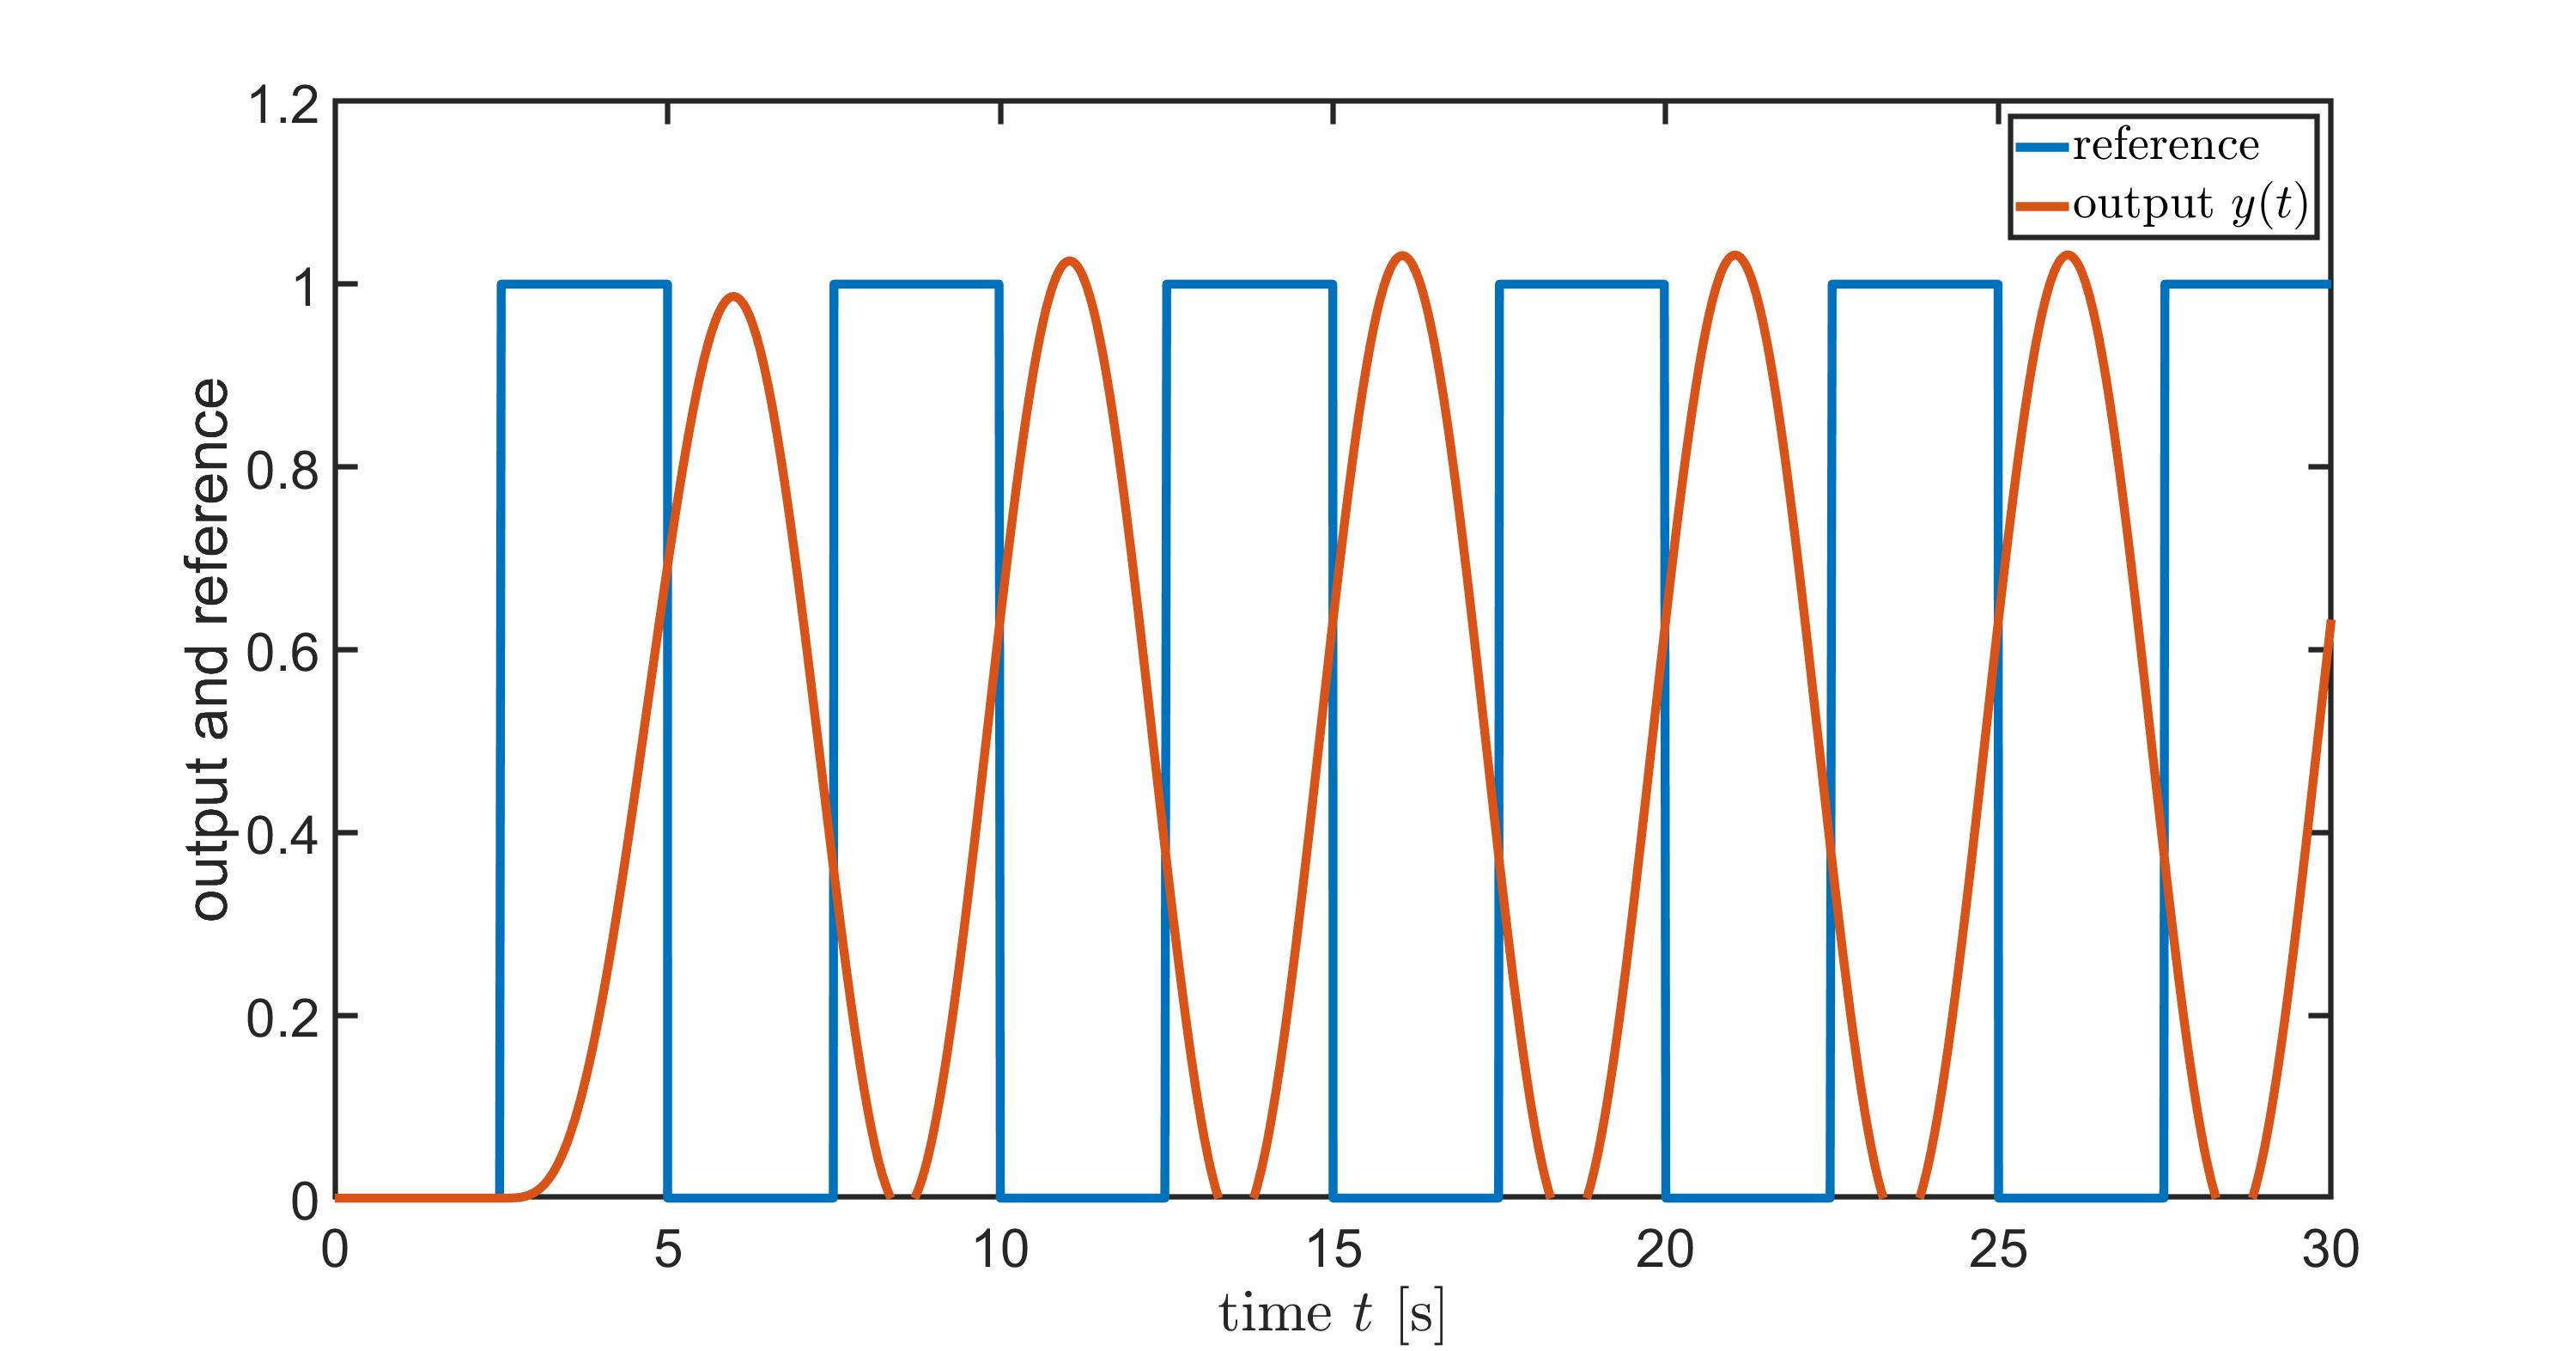
\includegraphics[width=\textwidth]{fig/ExSat_LQR.jpg}
		\caption{LQR Solution for the system \eqref{eq:Appl:satellite_sys}}
		\label{img:Appl:ExSat_LQR}
	\end{figure}
	
It looks like something we can improve. However, for $Ts = 10^{-3}$s we get $N = 10^3$ time steps even for one simulation second. The matrix $G$ has more than  $10^9$ elements and can not easily be handled.
\end{exam}

\section{Long time horizon}

	In Example \ref{ex:ILC:badIA} the Inverse Model Algorithm is not applicable even for $N = 50$. 
	It means, we need a trade off between the time horizon and robustness.
	However, for real problems the sample times are mostly small, and hence even for one second of the simulation we get huge number for time horizon. Already for SISO system the matrix $G$ will have $(N + 1)^2$ elements. Our algorithms become unusable for casual applications since they need vast masses of memory.	
	
	One possibility to reduce the wasted memory is to split our system in the smaller ones. Let us denote the time horizon length with $N_{\max}$, and choose an $N$ with $1<N\leq N_{\max}$. 
	We can apply our algorithms on the systems with the same state space description, but different initial values. For simplicity, let us assume, that we can divide our time horizon $0,1,2,\dots, N_{\max}$ in $p$ equal parts with time horizon of length $N$, and the matrix $D = 0$. 
	
	Then after we ran $N$ iterations, we get for the next $N$ iterations the initial condition
	\begin{align}
	x_{0_{\rm{1}}} = A^{N} x(0) + \sum_{\tau = 0}^N A^{\tau}B u(t - \tau). 
	\end{align}
	
	For the next pass we adjust the next initial value as 
	\begin{align}
	x_{0_{\rm{2}}} = A^{2N} x(0) + \sum_{\tau = 0}^{2N} A^{\tau}B u(t - \tau) = A^N x(N+1) + \sum_{\tau = 0}^N A^{\tau} B u(2N - \tau). 
	\end{align}
	
	Doing so fare $1 \leq p^* \leq p$ algorithm trials, we get 
	\begin{align}
	x_{0_{p^*}} = A^N x((N+1)(p^* - 1)) + \sum_{\tau = 0}^N A^{\tau}B u(p^*N - \tau). 
	\end{align}
	
	That means, we have no need to calculate even more than $N$ powers of $A$. 
	
	However, if the matrix is asymptotically stable, it might have an advantage to neglect some terms $C A^p B$ for $1<p<N$ large enough. 
	It allows us to skip the little elements of the matrix $G$, which might lead to bad condition number. 

	Another benefit is the use of sparse matrices. 	
	Our matrix $G$ has a lower triangular structure, and even without any neglecting we can decrease the memory usage by saving only the elements of $G$, which are not zero. With ''reduces'' matrix $G$ we can maintain more space and hence choose a larger $N$ to divide our system in.
	
	The following theorem illustrates it and supposes a method for choosing of this $p^*$. 
	
	\begin{theo}
	We consider the ''reduced'' lifted system 
	\begin{align}
	\t y = \t G + d.
	\end{align}
	The matrix 
	\begin{align}
	\t G = \begin{pmatrix}
	D  \\
	CB & D \\
	C A B & CB & D\\
	\vdots & \vdots & \vdots & \ddots \\
	C A^{p^\star-1} B & C A^{p^\star-2}B & C A^{p^\star-3}B &\dots& D \\
	0           & C A^{p^\star-1} B & C A^{p^\star-2} B & \dots & CB & D\\
	0 & 0 & C A^{p^\star-1} B & \dots & CAB & CB & D \\
	\vdots & \vdots & \vdots & \ddots & \vdots & \vdots & \vdots & \ddots \\
	0 & 0 & 0 & \dots & C A^{p^\star-1}& C A^{p^\star-2}B& CA^{p^\star-3}B &\dots & D
	\end{pmatrix},
	\end{align}
	with asymptotic stable $A$.
	
	Then the error $||y(t) - \t y(t)||$, $p^* < t$, can be estimated undepended on $t$ as 
	\begin{align}
	||y(t) - \t y(t)|| < 2 ||C|| \, ||B|| \,  ||A^{p^*}||\, ||(I - A)^{-1}||\,||u_{\max}||, 
	\end{align}
	with 
	\begin{align}
	||u_{\max}|| = \max_{\tau = 0}^{t - p^*} ||u(\tau)||. 
	\end{align}

	\end{theo}	
	\begin{proof}
	Since $A$ is asymptotically stable, the inverse of $(I - A)$ exists. Simple calculation provides 
		\begin{align}
	\begin{split}
			||y(t) - \t y(t)|| &= ||C \sum_{\tau = p^*}^t A^\tau B u(\tau)|| \leq ||C|| \, ||\sum_{\tau = p^*}^t A^\tau || \,||B|| \, ||u_{\max}|| \\
			& = ||C|| \, ||B|| \, ||(A^{p^*} - A^{t + 1})(I - A)^{-1}|| \, ||u_{\max}|| \\
			&  \leq 2 ||C|| \, ||B|| \, ||A^{p^*}|| \, ||(I - A)^{-1}|| \, ||u_{\max}||. 
	\end{split}
		\end{align}
	\end{proof}

	This theorem says, that it does not matter how large is our $N$: we still can estimate our output with the same $p^*$. 
	Thou this estimation is not very precise, and hence is not a good tool for any system. 
	
	
	
	
	
	
	
	